\documentclass[12pt]{article}
\usepackage{hyperref}
\usepackage{graphicx}
\usepackage{caption}
\usepackage{geometry}
\usepackage{float}
\usepackage{amsmath}
\usepackage{algorithm}
\usepackage{algpseudocode}
\usepackage{tikz}
\usepackage{enumitem}
\usepackage{tabularx}
\usepackage{makecell}
\usepackage{biblatex}
\usepackage{appendix}
\usepackage{subcaption}
\usepackage{listings}
\usepackage{wrapfig}
\usepackage{ragged2e}
\usepackage{booktabs}
\usepackage{pgfplots}

\addbibresource{bibliography.bib}

\geometry{a4paper, margin=1.5cm}
\setlength{\parindent}{0em}
\setlength{\parskip}{0.5em}

\begin{document}

\begin{titlepage}
    \centering
    \vspace*{3cm}
    {\Huge\bfseries Compound Pendulum: A Delivery Exercise in Fuzzy Computing\par}
    \vspace{1.5cm}
    {\large Mauro V\'AZQUEZ CHAS, D\'aniel M\'ACSAI \par}
    \vspace{3cm}
    {\large \textbf{Master in Artificial Intelligence}\par}
    
\includegraphics[width=0.4\textwidth]{Logo_UPC.png}\par\vspace{1cm}
    {\large \textbf{Planning and Approximate Reasoning}\par}
    \vspace{1cm}
    {\large\bfseries 10th January 2024\par}
\end{titlepage}

\pagestyle{empty}

\newpage
\tableofcontents
\newpage

% Set page numbering    
\setcounter{page}{1}
\pagestyle{plain}

\section{Introduction}
\label{sec:introduction}

The compound pendulum models robotic arm movement, important for control systems and mechanical modeling. It consists of a uniform bar with mass \( m \) and length \( l \), suspended at a sliding pivot point \( A \), adjustable by distance \( h \) from the center of gravity. This configuration, combined with a motor and propeller, results in oscillations requiring advanced control for stabilization.

This report focuses on designing a Mamdani fuzzy inference system (FIS) controller using Simulink and MATLAB’s fuzzy toolbox to improve the pendulum’s transient response and stabilize its angular position. The open-loop response shows sustained oscillations, highlighting the need for feedback control. Real-time angle measurements from an encoder are used for implementing control strategies.

The report covers defining fuzzy membership functions for error, error derivative, and thrust, establishing a rule base, and simulating the system’s behavior. It also compares fuzzy control with the open-loop system and explores the impact of refining membership function granularity.

\section{Design of the Fuzzy Controller}
\label{sec:design}

\subsection{Membership Functions}

Here we provide the membership functions we used for the fuzzy controller. We have three input variables: Error, Error Derivative, and one output variable, the Thrust. 

\subsubsection{Error}

The error variable represents the difference between the desired and actual angular position of the pendulum. Following the instructions, we defined the membership functions as detailed below:

\begin{figure}[H]
    \centering
    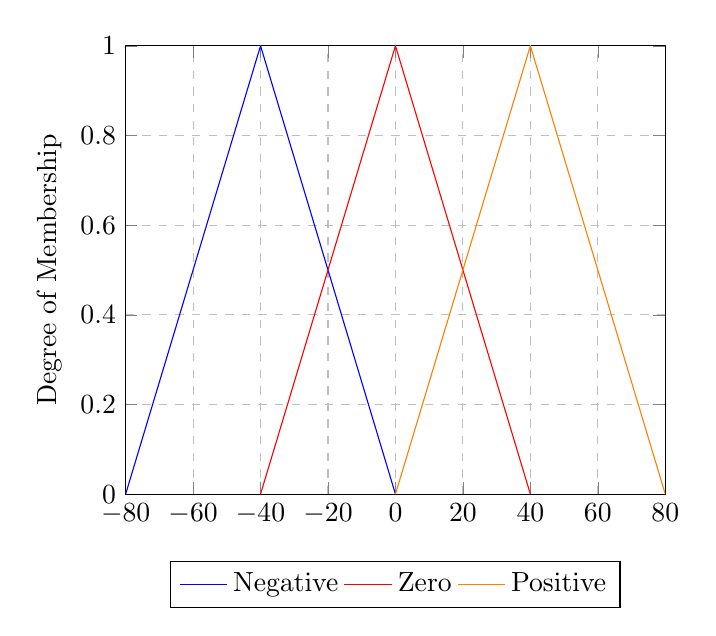
\begin{tikzpicture}
        \begin{axis}[
            ylabel={Degree of Membership},
            ymin=0, ymax=1,
            xmin=-80, xmax=80,
            legend style={at={(0.5,-0.15)},anchor=north,legend columns=-1},
            ymajorgrids=true,
            xmajorgrids=true,
            grid style=dashed
        ]
        
        % Negative Membership Function
        \addplot[solid, blue] coordinates {(-80,0) (-40,1) (0,0)};
        \addlegendentry{Negative}
        
        % Zero Membership Function
        \addplot[solid, red] coordinates {(-40,0) (0,1) (40,0)};
        \addlegendentry{Zero}
        
        % Positive Membership Function
        \addplot[solid, orange] coordinates {(0,0) (40,1) (80,0)};
        \addlegendentry{Positive}
        
        \end{axis}
    \end{tikzpicture}
    \caption{Membership Functions for Input Variable "Error"}
\end{figure}

We believe this variable could model reality more accurately using trapezoidal membership functions for the lowest and highest values. For instance, when the error exceeds 40 degrees, the corresponding membership function starts decreasing, which might influence rule activation. However, we adhered to the instructions and used triangular membership functions.

\subsubsection{Error Derivative}

\begin{figure}[H]
    \centering
    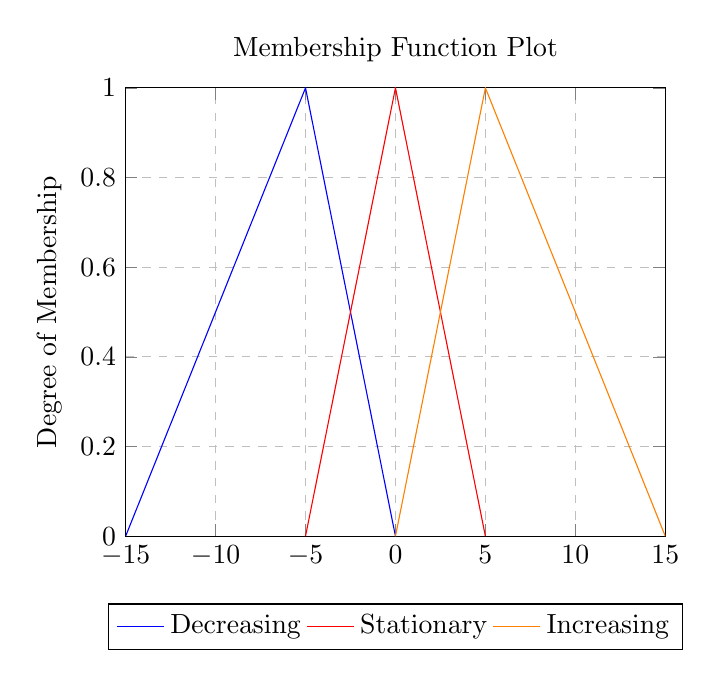
\begin{tikzpicture}
        \begin{axis}[
            title={Membership Function Plot},
            ylabel={Degree of Membership},
            ymin=0, ymax=1,
            xmin=-15, xmax=15,
            legend style={at={(0.5,-0.15)},anchor=north,legend columns=-1},
            ymajorgrids=true,
            xmajorgrids=true,
            grid style=dashed
        ]
        
        % Decreasing Membership Function
        \addplot[solid, blue] coordinates {(-15,0) (-5,1) (0,0)};
        \addlegendentry{Decreasing}
        
        % Stationary Membership Function
        \addplot[solid, red] coordinates {(-5,0) (0,1) (5,0)};
        \addlegendentry{Stationary}
        
        % Increasing Membership Function
        \addplot[solid, orange] coordinates {(0,0) (5,1) (15,0)};
        \addlegendentry{Increasing}
        
        \end{axis}
    \end{tikzpicture}
    \caption{Membership Functions for Input Variable "Error Derivative"}
\end{figure}

The same observation applies to the Error Derivative variable. Initially, the range was set to [-5, 5], but during simulations, the derivative often exceeded these bounds, causing the fuzzy controller to output zero. We adjusted the range to [-15, 15] for improved results.

\subsubsection{Thrust}

\begin{figure}[H]
    \centering
    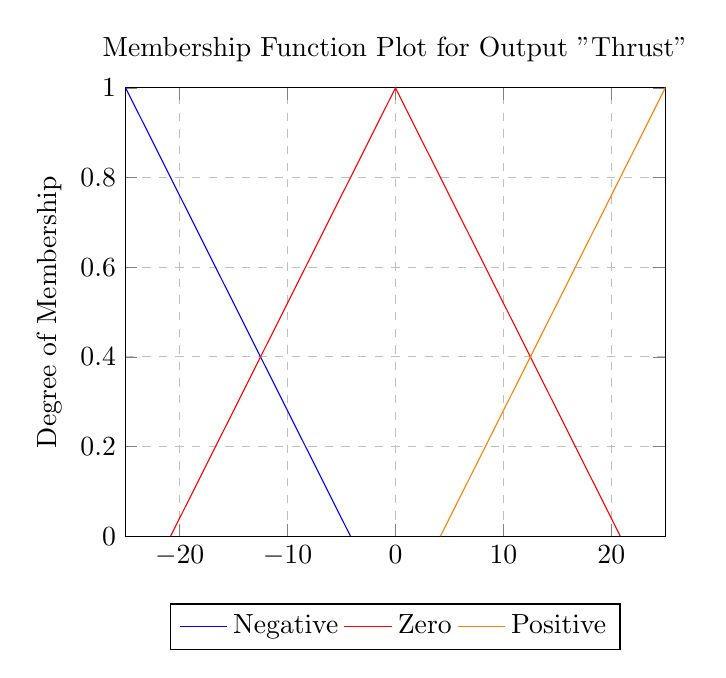
\begin{tikzpicture}
        \begin{axis}[
            title={Membership Function Plot for Output "Thrust"},
            ylabel={Degree of Membership},
            ymin=0, ymax=1,
            xmin=-25, xmax=25,
            legend style={at={(0.5,-0.15)},anchor=north,legend columns=-1},
            ymajorgrids=true,
            xmajorgrids=true,
            grid style=dashed
        ]
        
        % Negative Membership Function
        \addplot[solid, blue] coordinates {(-45.833,0) (-25,1) (-4.167,0)};
        \addlegendentry{Negative}
        
        % Zero Membership Function
        \addplot[solid, red] coordinates {(-20.833,0) (0,1) (20.833,0)};
        \addlegendentry{Zero}
        
        % Positive Membership Function
        \addplot[solid, orange] coordinates {(4.167,0) (25,1) (45.833,0)};
        \addlegendentry{Positive}
        
        \end{axis}
    \end{tikzpicture}
    \caption{Membership Functions for Output Variable "Thrust"}
\end{figure}

Since the design of this variable was not provided, we made the Negative and Positive variables activate at the highest levels for the lowest and highest values, respectively. The three variables are evenly distributed across the interval \([-25, 25]\).

\subsection{Rules}

We designed the 9 rules required for this exercise as follows:

\begin{table}[h!]
    \centering
    \renewcommand{\arraystretch}{1.25} % Increase vertical space between rows
    \setlength{\tabcolsep}{10pt}      % Increase horizontal space between columns
    \begin{tabular}{|p{3cm}|p{4cm}|p{3cm}|}
    \hline
    \textbf{\large Error} & \textbf{\large ErrorDerivative} & \textbf{\large Thrust} \\ \hline
    \large Negative       & \large Decreasing                & \large Negative        \\ \hline
    \large Zero           & \large Decreasing                & \large Negative        \\ \hline
    \large Positive       & \large Decreasing                & \large Positive        \\ \hline
    \large Negative       & \large Stationary                & \large Negative        \\ \hline
    \large Zero           & \large Stationary                & \large Zero            \\ \hline
    \large Positive       & \large Stationary                & \large Positive        \\ \hline
    \large Negative       & \large Increasing                & \large Negative        \\ \hline
    \large Zero           & \large Increasing                & \large Positive        \\ \hline
    \large Positive       & \large Increasing                & \large Positive        \\ \hline
    \end{tabular}
    \caption{Rules and Corresponding Weights}
    \label{tab:rules}
\end{table}

When the Error is not \textit{Zero}, the Thrust is set accordingly: if the Error is \textit{Negative}, the Thrust is \textit{Negative}; if the Error is \textit{Positive}, the Thrust is \textit{Positive}. The Error Derivative variable is used to fine-tune the Thrust. For instance, if the Error is \textit{Zero} but \textit{Increasing}, the Thrust is \textit{Positive}; if the Error is \textit{Decreasing}, the Thrust is \textit{Negative}. When both Error and Error Derivative are \textit{Zero}, the Thrust is set to \textit{Zero}.

\section{Results}

We ran the simulation for a stop time of 80 seconds using the provided controller and parameters. The results are shown in figures \ref{fig:simulation1} and \ref{fig:simulation2}. 

\begin{figure}[h!]
    \centering
    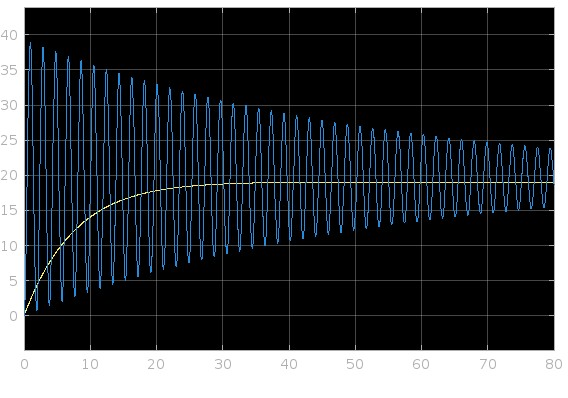
\includegraphics[width=0.7\textwidth]{simulation1.jpg}
    \caption{theta\_ref = 20 and thrust = 0.123}
    \label{fig:simulation1}
\end{figure}

\begin{figure}[h!]
    \centering
    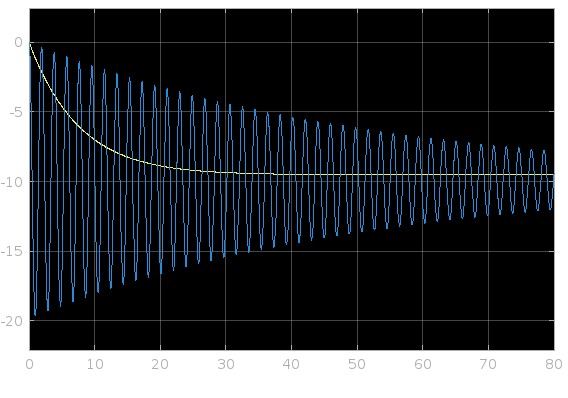
\includegraphics[width=0.7\textwidth]{simulation2.jpg}
    \caption{theta\_ref = -10 and thrust = -0.062}
    \label{fig:simulation2}
\end{figure}

In both cases, our designed control system was able to stabilize the pendulum at the desired angle. We don't see any oscillations, and the system reaches the desired angle in a reasonable time. We can clearly see how the thrust is adjusted according to the error and its derivative. 

\section{More complex controller}

To test out the cababilities of the fuzzy controller, we designed a more complex controller with 7 membership functions for the Thrust output variable. The plots frim the simulation are shown in figures \ref{fig:complex1} and \ref{fig:complex2}.

\begin{figure}[H]
    \centering
    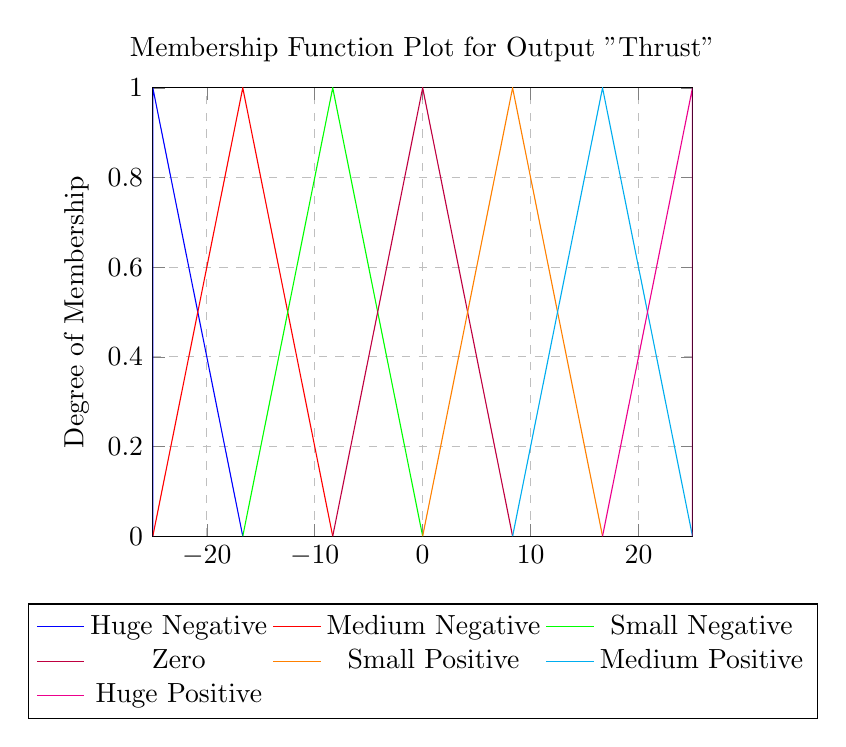
\begin{tikzpicture}
        \begin{axis}[
            title={Membership Function Plot for Output "Thrust"},
            ylabel={Degree of Membership},
            ymin=0, ymax=1,
            xmin=-25, xmax=25,
            legend style={at={(0.5,-0.15)},anchor=north,legend columns=3},
            ymajorgrids=true,
            xmajorgrids=true,
            grid style=dashed
        ]
        
        % Huge Negative Membership Function
        \addplot[solid, blue] coordinates {(-25,0) (-25,1) (-16.6667,0)};
        \addlegendentry{Huge Negative}
        
        % Medium Negative Membership Function
        \addplot[solid, red] coordinates {(-25,0) (-16.6667,1) (-8.3333,0)};
        \addlegendentry{Medium Negative}
        
        % Small Negative Membership Function
        \addplot[solid, green] coordinates {(-16.6667,0) (-8.3333,1) (0,0)};
        \addlegendentry{Small Negative}
        
        % Zero Membership Function
        \addplot[solid, purple] coordinates {(-8.3333,0) (0,1) (8.3333,0)};
        \addlegendentry{Zero}
        
        % Small Positive Membership Function
        \addplot[solid, orange] coordinates {(0,0) (8.3333,1) (16.6667,0)};
        \addlegendentry{Small Positive}
        
        % Medium Positive Membership Function
        \addplot[solid, cyan] coordinates {(8.3333,0) (16.6667,1) (25,0)};
        \addlegendentry{Medium Positive}
        
        % Huge Positive Membership Function
        \addplot[solid, magenta] coordinates {(16.6667,0) (25,1) (25,0)};
        \addlegendentry{Huge Positive}
        
        \end{axis}
    \end{tikzpicture}
    \caption{Membership Functions for Output Variable "Thrust"}
\end{figure}

To make a change, we need to modify the rules too. Here are the updated rules:

\begin{table}[h!]
    \centering
    \renewcommand{\arraystretch}{1.25} % Increase vertical space between rows
    \setlength{\tabcolsep}{10pt}      % Increase horizontal space between columns
    \begin{tabular}{|p{3cm}|p{4cm}|p{5cm}|}
    \hline
    \textbf{\large Error} & \textbf{\large ErrorDerivative} & \textbf{\large Thrust} \\ \hline
    \large Negative       & \large Decreasing               & \large Huge Negative    \\ \hline
    \large Zero           & \large Decreasing               & \large Small Negative   \\ \hline
    \large Positive       & \large Decreasing               & \large Medium Negative  \\ \hline
    \large Negative       & \large Stationary               & \large Medium Negative  \\ \hline
    \large Zero           & \large Stationary               & \large Zero             \\ \hline
    \large Positive       & \large Stationary               & \large Medium Positive  \\ \hline
    \large Negative       & \large Increasing               & \large Medium Negative  \\ \hline
    \large Zero           & \large Increasing               & \large Small Positive   \\ \hline
    \large Positive       & \large Increasing               & \large Huge Positive    \\ \hline
    \end{tabular}
    \caption{Fuzzy Logic Rules for Thrust Calculation}
    \label{tab:rules}
\end{table}

Both simulations were conducted using the new controller, and the results are presented in the following figures:

\begin{figure}[h!]
    \centering
    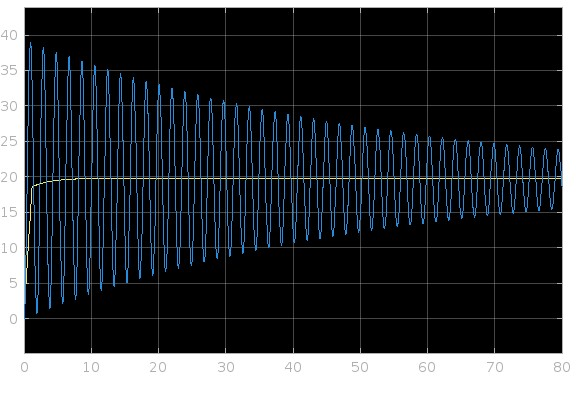
\includegraphics[width=0.7\textwidth]{complex1.jpg}
    \caption{theta\_ref = 20 and thrust = 0.123}
    \label{fig:complex1}
\end{figure}

\begin{figure}[h!]
    \centering
    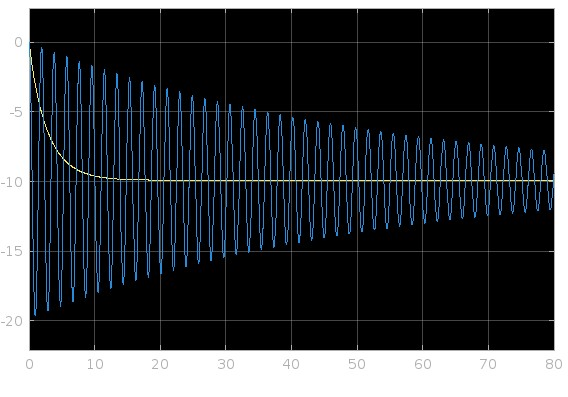
\includegraphics[width=0.7\textwidth]{complex2.jpg}
    \caption{theta\_ref = -10 and thrust = -0.062}
    \label{fig:complex2}
\end{figure}

Initially, it was hypothesized that improvements would require increasing the sensitivity of the input variables by incorporating additional membership functions and more complex rules. However, a significant improvement was observed by modifying only the output variable. This adjustment enabled the system to reach the desired angle more rapidly while maintaining stability. While further optimization of the input variables could enhance performance, the current results are already highly promising.

\section{Conclusions}  

    In this study, we successfully designed and implemented a Mamdani fuzzy inference system (FIS) to control a compound pendulum, achieving significant improvements in stability and transient response compared to the open-loop system. The fuzzy controller effectively reduced oscillations and achieved the desired angular position, demonstrating robustness and adaptability. By experimenting with enhanced membership functions and a more granular rule base, we observed that increasing the complexity of the output variable improved response speed and stability without requiring additional adjustments to input variables. This highlights the potential of fuzzy logic systems to handle nonlinear control problems efficiently. The results underscore the versatility and practicality of fuzzy computing in real-world dynamic systems.

\section{Usage of generative AI models}

We used ChatGPT for spelling checks, grammar corrections, and sentence structure improvements. 

\end{document}